\begin{figure}[htbp]
  \centering
  \begin{tikzpicture}[
      node distance=2cm,
      block/.style={draw, rectangle, minimum width=2cm, minimum
      height=1.5cm, align=center},
      arrow/.style={->, >=stealth, thick},
      label/.style={font=\small}
    ]

    % Main image concept
    \node[block] (main) {Digital Image};
    \node[block, below left=of main] (grayscale) {Grayscale};
    \node[block, below=of main] (color) {Color};
    \node[block, below right=2.5cm and 1cm of main] (multispectral)
    {Multispectral};
    \node[block, below right=1cm and 3.5cm of main] (volumetric)
    {3D/Volumetric};

    % Mathematical representations
    \node[block, below=of grayscale] (gray_math) {2D Matrix\\$M \times N$};
    \node[block, below=of color] (color_math) {3D Matrix\\$M \times N
    \times 3$};
    \node[block, below=of multispectral] (multi_math) {3D Matrix\\$M
    \times N \times B$};
    \node[block, below=of volumetric] (vol_math) {3D Matrix\\$M
    \times N \times D$};

    % Sampling and quantization
    \node[block, left=of main] (sampling) {Sampling};
    \node[block, right=of main] (quantization) {Quantization};

    % Connect main concept to types
    \draw[arrow] (main) -- (grayscale);
    \draw[arrow] (main) -- (color);
    \draw[arrow] (main) -- (multispectral);
    \draw[arrow] (main) -- (volumetric);

    % Connect types to mathematical representations
    \draw[arrow] (grayscale) -- (gray_math);
    \draw[arrow] (color) -- (color_math);
    \draw[arrow] (multispectral) -- (multi_math);
    \draw[arrow] (volumetric) -- (vol_math);

    % Connect sampling and quantization
    \draw[arrow] (sampling) -- (main);
    \draw[arrow] (quantization) -- (main);

    % Add labels
    \node[label, above=0.5cm of main] {Digital Image Concepts};
    \node[label, above=0.5cm of sampling] {Processes};
    \node[label, above=0.5cm of quantization] {Processes};

    % Add example images placeholders
    \node[draw, rectangle, minimum width=2cm, minimum height=1.5cm,
    below=0.5cm of gray_math] (gray_ex)
    {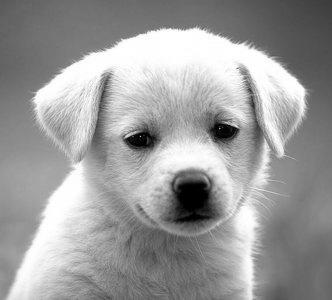
\includegraphics[width=2cm]{Cap2/Figures/gray_example.jpg}};
    \node[draw, rectangle, minimum width=2cm, minimum height=1.5cm,
    below=0.5cm of color_math] (color_ex)
    {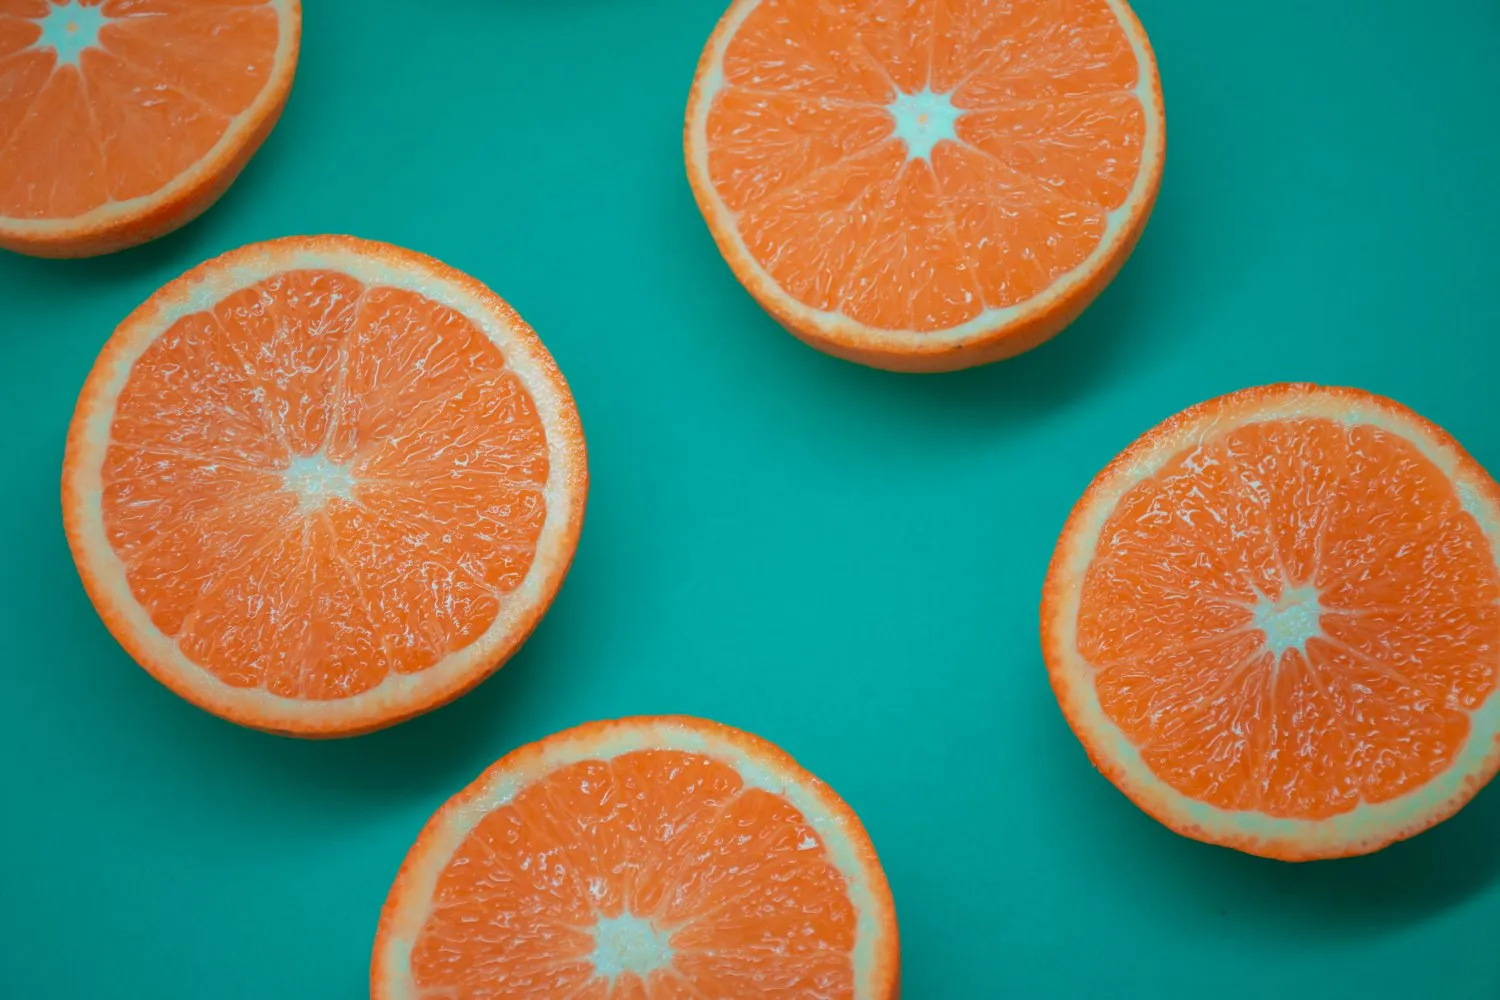
\includegraphics[width=2cm]{Cap2/Figures/color_example.png}};
    \node[draw, rectangle, minimum width=2cm, minimum height=1.5cm,
    below=0.5cm of multi_math] (multi_ex)
    {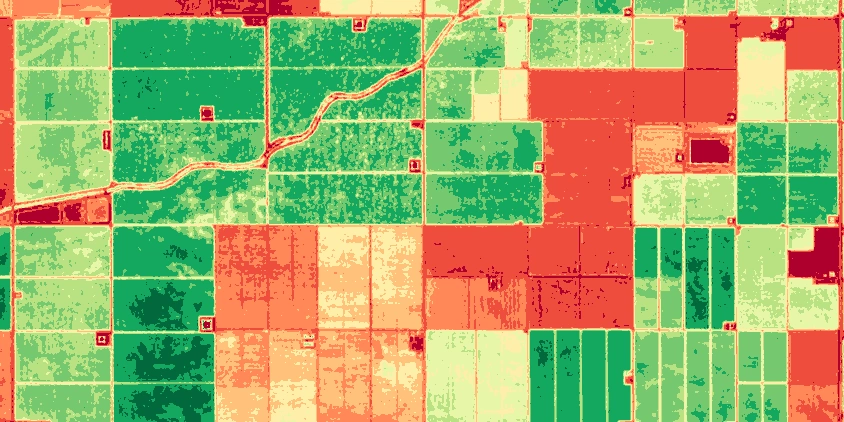
\includegraphics[width=2cm]{Cap2/Figures/multispectral_example.png}};
    \node[draw, rectangle, minimum width=2cm, minimum height=1.5cm,
    below=0.5cm of vol_math] (vol_ex)
    {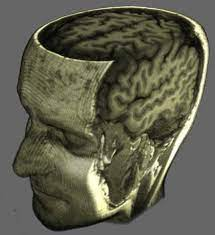
\includegraphics[width=2cm]{Cap2/Figures/volumetric_example.jpg}};

    % Connect mathematical representations to examples
    \draw[arrow] (gray_math) -- (gray_ex);
    \draw[arrow] (color_math) -- (color_ex);
    \draw[arrow] (multi_math) -- (multi_ex);
    \draw[arrow] (vol_math) -- (vol_ex);

  \end{tikzpicture}
  \caption{Overview of digital image concepts and their mathematical
    representations. The figure shows the main types of digital images
    (grayscale, color, multispectral, and volumetric), their
    mathematical representations, and the fundamental processes of
    sampling and quantization. Example images are included to
  illustrate each type.}
  \label{fig:image_concepts}
\end{figure}